\documentclass[a4paper,abstracton]{scrreprt}
\usepackage[T1]{fontenc}
\usepackage[utf8]{inputenc}
\usepackage[ngerman]{babel}
\usepackage{pdfpages} 

%correct linebreaking in bibliography
\usepackage{hyperref}
\usepackage{breakurl}

%Formatierung des Inhaltsverzeichnisses
\usepackage{tocloft}
\cftsetindents{chapter}{0in}{0.5in}
\cftsetindents{section}{0in}{0.5in}
\cftsetindents{subsection}{0in}{0.5in}
\setlength\cftbeforechapskip{18pt}


%pictures
\usepackage{float}
\usepackage{graphicx}
\graphicspath{{img/}}

%biblatex
\usepackage[babel,german=quotes]{csquotes}
\usepackage[style=authortitle]{biblatex}

\bibliography{literatur}
\defbibheading{lit}{\chapter{Literaturverzeichnis}}
\setlength\bibitemsep{2\itemsep}

\usepackage{filecontents}
\begin{filecontents}{literatur.bib} 
@Electronic{hikersnotebook:oystermushroom,
  Title                    = {Übersetung Pleurotus},
  Author                   = {hikersnotebook.net},
  Url                      = {http://hikersnotebook.net/Oyster+Mushroom},
  Note                     = {Navigation: Suche, Oyster Mushroom},
  Urldate				   = {2014-07-05}
}
@Electronic{duden:seitlinge,
  Title                    = {Definition Seitlinge},
  Author                   = {duden.de},
  Url                      = {http://www.duden.de/suchen/dudenonline/Seitling},
  Note                     = {Navigation: Suche, Seitling, erster Treffer},
  Urldate				   = {2014-08-10}
}
@Electronic{enzyklo:seitlinge,
  Title                    = {Definition Seitlinge},
  Author                   = {enzyklo.de},
  Url                      = {http://www.enzyklo.de/Begriff/Seitlinge},
  Note                     = {Navigation: Definitionen, Suche, Seitlinge},
  Urldate				   = {2014-07-05}
}
@Electronic{pilzech,
	Title					= {Pilzbestimmung Pleurotus},
	Author					= {pilze.ch},
	Url						= {http://www.pilze.ch/pilzbestimmung/artenlisten/Pleurotus.htm},
	Keywords				= {pilze.ch},
	Note					= {Navigation: Pilzbestimmung, Gattungen und Arten, Pleurotus},
	Urldate					= {2014-07-05}
}
@Electronic{pg_austernseitling,
	Title					= {Pilzgalerie Austernseitling},
	Author					= {123pilze.de},
	Url						= {http://www.123pilze.de/DreamHC/Download/Austernseitling1105.htm},
	Keywords				= {www.123pilze.de},
	Note					= {Navigation: Pilze nach Alphabet geordnet, Austernseitling},
	Urldate					= {2014-07-05}
}
@Electronic{vital,
	Title					= {Vitalpilzratgeber},
	Author					= {vitalpilzratgeber.de},
	Url						= {http://www.vitalpilzratgeber.de/pleurotus/},
	Keywords				= {www.vitalpilzratgeber.de},
	Note					= {Navigation: Pleurotus},
	Urldate					= {2014-07-05}
}
@Electronic{pg_ohrfoermig,
	Title					=  {Pilzgalerie Ohrförmiger Seitling},
	Author					= {123pilze.de},
	Url						= {http://www.123pilze.de/DreamHC/Download/OhrfoermigerSeitling.htm},
	Keywords				= {www.123pilze.de},
	Note					= {Navigation: Pilze nach Alphabet geordnet, Ohrförmiger Seitling},
	Urldate					= {2014-07-06}
}
@Online{deutschlandradio,
	Title					= {Speisepilz wird Giftpilz},
	Author					= {Udo POLLMER},
	month = jun,
	year = {2008},
	Url						= {http://www.deutschlandradiokultur.de/speisepilz-wird-giftpilz.993.de.html?dram:article_id=154417},
	Keywords				= {www.deutschlandradiokultur.de},
	Note					= {Navigation: Suche nach \emph{Speisepilz wird Giftpilz}, Ohrförmiger Seitling},
	Urldate					= {2014-07-06}
}
@Electronic{tintling_auster,
	Title					= {Austernseitling Pleurotus ostreatus},
	Author					= {tintling.com},
	Url						= {http://tintling.com/pilzbuch/arten/p/Pleurotus_ostreatus.html},
	Keywords				= {www.tintling.com},
	Note					= {Navigation: Pilzbuch, Gattungen, Pleurotus,  Pleurotus ostreatus},
	Urldate					= {2014-07-06}
}
@Electronic{tintling_kraeuter,
	Title					=  {Brauner Kräuter-SeitlingPleurotus eryngii},
	Author					= {tintling.com},
	Url						= {http://tintling.com/pilzbuch/arten/p/Pleurotus_eryngii.html},
	Keywords				= {www.tintling.com},
	Note					= {Navigation: Pilzbuch, Gattungen, Pleurotus,  Pleurotus eryngii},
	Urldate					= {2014-07-06}
}
@Electronic{tintling_berindet,
	Title					=  {Berindeter Seitling Pleurotus dryinus},
	Author					= {tintling.com},
	Url						= {http://tintling.com/pilzbuch/arten/p/Pleurotus_dryinus.html},
	Keywords				= {www.tintling.com},
	Note					= {Navigation: Pilzbuch, Gattungen, Pleurotus,  Pleurotus dryinus},
	Urldate					= {2014-07-08}
}
@Electronic{tintling:lungenseitling,
	Title					= {Lungenseitling, Löffel-Seitling Pleurotus pulmonarius},
	Author					= {tintling.com},
	Url						= {http://tintling.com/pilzbuch/arten/p/Pleurotus_pulmonarius.html},
	Keywords				= {www.tintling.com},
	Note					= {Navigation: Pilzbuch, Gattungen, Pleurotus,  Pleurotus pulmonarius},
	Urldate					= {2014-08-11}
}
@Electronic{rezept,
	Title					= {Kräuterseitlinge mit Nudeln},
	Author					= {SIMU},
	Url						= {http://www.kochbar.de/rezept/314872/Kraeuterseitlinge.html},
	Keywords				= {www.kochbar.de},
	Note					= {Navigation: Suche nach \emph{Kräuterseitlinge}, zweites Rezept},
	month = mar,
	year = {2010},
	day = {12},
	Urldate					= {2014-07-08}
}
@online{pilzfinder_austernseitling_image,
	Title					= {Austernseitling},
	Author					= {Jürgen MATHES},
	Url						= {http://www.pilzfinder.de/highlight/auster2.jpg},
	Keywords				= {www.pilzfinder.de},
	Note					= {Navigation: Pilze von A -- Z, Austernseitling, oberstes Bild},
	month = jan,
	year = {2012},
	day = {1},
	Urldate					= {2014-07-06}
}
@online{tintling:kraeuterseitling_image,
	Title					= {Brauner Kräuter-Seitling},
	Author					= {Markus WILHELM},
	Url						= {http://www.tintling.com/pilzbuch/pilzbilder/Pleurotus_eryngii.jpg},
	Keywords				= {http://www.tintling.com/},
	Note					= {Navigation: Pilzbuch, Gattungen, Pleurotus,  Pleurotus eryngii},
	Urldate					= {2014-08-06}
}
@online{fotocom_berindeter_seitling_image,
	Title					= {Berindeter Seitling -- Fotocommunity},
	Author					= {Wolfgang ZEISELMAIR},
	Url						= {http://www.fotocommunity.de/search?q=Berindeter+seitling&index=fotos&options=YToxOntzOjU6InN0YXJ0IjtpOjA7fQ&display=29319786},
	Keywords				= {www.fotocommunity.de},
	Note					= {Navigation: Suche, Suche nach \emph{Berindeter Seitling}, erstes Foto in der Übersicht},
	month = oct,
	year = {2012},
	day = {2},
	Urldate					= {2014-07-08}
}
@online{tintling:lungenseitling_image,
	Title					= {Lungenseitling},
	Author					= {Klaus RÖDDER},
	Url						= {http://tintling.com/pilzbuch/pilzbilder/Pleurotus_pulmonarius.jpg},
	Keywords				= {http://www.tintling.com/},
	Note					= {Navigation: Pilzbuch, Gattungen, Pleurotus,  Pleurotus pulmonarius},
	Urldate					= {2014-08-10}
}
@online{rezept_image,
	Title					= {zubereitete Kräuterseitlinge mit Nudeln},
	Author					= {SIMU},
	Url						= {http://autoimg.kochbar.de/kbrezept/314872_256625/400x266/rezept-kraeuterseitlinge-bild-nr-7.jpg},
	Keywords				= {www.kochbar.de},
	Note					= {Navigation: Suche nach \emph{Kräuterseitlinge}, zweites Rezept, Bild Nr. 7},
	month = mar,
	year = {2010},
	day = {12},
	Urldate					= {2014-07-08}
}
\end{filecontents} 

%set numeration depth
\setcounter{secnumdepth}{3}
%set how many numbers show up in table-of-contents
\setcounter{tocdepth}{2}
\setlength{\parindent}{0em} 
%Rand oben
\usepackage{geometry}
 \geometry{
 a4paper,
 top=20mm
 }
\renewcommand*\chapterheadstartvskip{\vspace*{0cm}}



\begin{document}
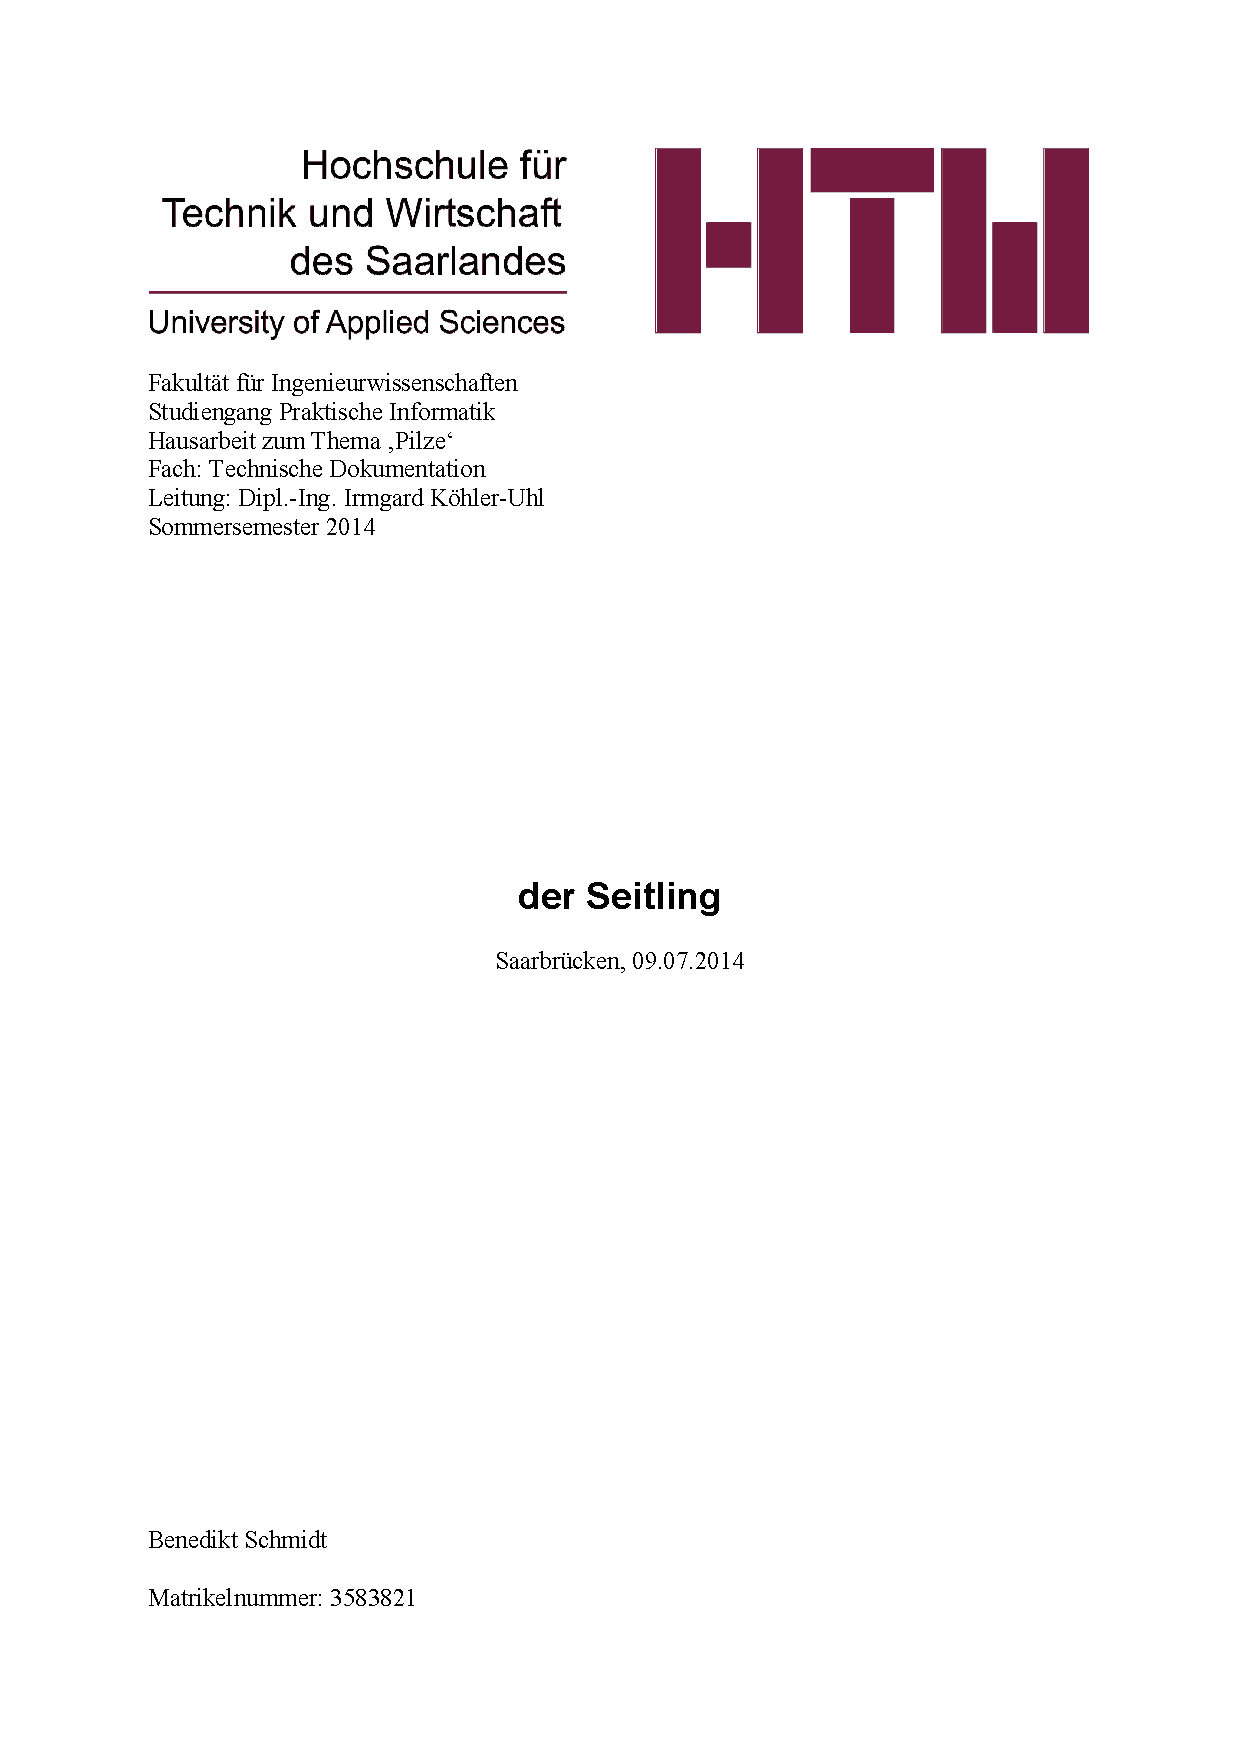
\includepdf[]{Deckblatt_Seitling.pdf}

%\author{Benedikt Schmidt}
%\subject{Pilze}
%\title{der Seitling}
%\publishers{htwsaar}
%\maketitle
\tableofcontents
\pagebreak
\listoffigures
%\listoftables

\begin{abstract}
\begin{quote}%abstand rechts und links
Unter dem Schirmthema \emph{Heimische Pilze} beschäftigt sich diese Ausarbeitung mit den Seitlingen (lat.: "'Pleurotus"'). Es werden unter anderem Kenntnisse über Allgemeinheiten, das Vorkommen, die Beschreibung des Pilzes sowie die bei Pilzen so wichtigen Verwechslungsmöglichkeiten vermittelt. Weiterhin wird eine Auswahl ausgesuchter Arten einzeln betrachtet.
\end{quote} 
\end{abstract}

\chapter{Vorwort}
Diese Ausarbeitung ist Bestandteil einer Reihe von Ausarbeitungen, die im Zuge der Vorlesung "'Technische Dokumentation"' entstanden sind. Der Kerngedanke bei der Anfertigung dieser Arbeit ist, zu erlernen, wie man mit fachbezogenen Texten umgeht -- von der Recherche über die Erstellung bis hin zur Anfertigung eines korrekten Literaturverzeichnisses. 

\chapter{Der Seitling}
\section{Allgemeines}
Die Seitlinge (lat. \emph{Pleurotus}) sind eine Pilzgattung aus der Familie der Seitlingsverwandten.  Der lateinische Name \emph{Pleurotus} leitet sich von griechisch \emph{pleura} = die Seite, und griechisch \emph{us} = das Ohr ab, da die Pilze oft ohrförmig sind und meist einen seitlichen Stiel besitzen. Der Stiel kann sich dabei auch am Rand befinden oder ganz fehlen. Der bekannteste Vertreter ist der Austernpilz.\footcite{hikersnotebook:oystermushroom} \footcite{enzyklo:seitlinge} \footcite{duden:seitlinge}

\section{Vorkommen}
Da Seitlinge eine große Gattung darstellen, wachsen diese auch an unterschiedlichsten Orten und unter verschiedenen Bedingungen. Sie sind auch nicht unbedingt zu einer ganz speziellen Jahreszeit anzutreffen. Viele Arten wachsen vorrangig zwischen Sommer und Herbst, einige sind jedoch auch im Winter zu sichten, wie zum Beispiel der Gemeine Orangenseitling (lat. \emph{Phyllotopsis nidulans}). Andere Arten wachsen bereits im Frühjahr, wie zum Beispiel der Lungenseitling(lat. \emph{Pleurotus pulmonarius}). Seitlinge wachsen meist auf Holz, teilweise aber auch auf Erde, Stroh oder toten Blättern. Dabei sind sie hauptsächlich auf totem Laub- oder Nadelholz, bzw. an morschem Bauholz anzutreffen.\footcite{pilzech}

\section{Beschreibung}
Bei den Seitlingen handelt es sich meist um seitlich wachsende Pilze mit kurzem beziehungsweise ohne Stiel. Ihre Hüte sind muschel-, nieren- oder halbkreisförmig. Die Hutunterseite wird durch helle, ganzrandige Lamellen gebildet. Sie laufen dem Stiel entlang herab. Die Hutoberseite hingegen ist kahl und nicht geschuppt. Sie ist ockerlich bis grau, graublau, grünlichgrau und glatt. Das Sporenpulver ist weiß und in seltenen Fällen etwas lila. Das Fleisch der Seitlinge hat bei jungen Fruchtkörpern eine saftige, alt bald eine zähle Konsistenz.\footcite{pilzech}\\
\\Die meisten Seitlinge sind nicht für den Verzehr geeignet. Einige Pilze, wie zum Beispiel der Austernseitling (lat. \emph{Pleurotus ostreatus}) sind jedoch als Speisepilze anerkannt.\footcite{pg_austernseitling}

\section{Arten}
Die Gattung Pleurotus umfasst mehr als 20 Arten. Da viele keine Speisepilze sind, sind die meisten jedoch relativ unbekannt.\footcite{pilzech} Im folgenden sollen die bekanntesten Vertreter der Gattung kurz beschrieben werden.

\subsection{Austernseitling}
Der im Durchmesser 5 bis 20 cm große Austernseitling ist der wohl bekannteste Vertreter der Seitlinge. Der Speisepilz kommt vorzugsweise an Rotbuchen vor, aber auch an vielen anderen Bäumen und sogar auf Stroh. In Mitteleuropa ist er recht häufig anzutreffen. Seine Hüte sind muschelförmig, meistens ohne deutlich abgesetzten Stiel. Seine Oberfläche ist glatt, feucht und fett glänzend, seine Farbe reicht von schiefergrau über blaugrau bis graubraun. Die Lamellen sind weiß, dünn und engstehend. Sein Fleisch ist dick, fest und im Stiel zäh.\\
\\Im Vergleich zu anderen Pilzarten ist der Austernseitling auch unter winterlichen Bedingungen noch zu finden. Er ist einer der bei uns am häufigsten angebotenen Kulturspeisepilze. Sein Geruch und Geschmack sind pilzartig-aromatisch.\footcite{tintling_auster}

\begin{figure}[H]
\centering
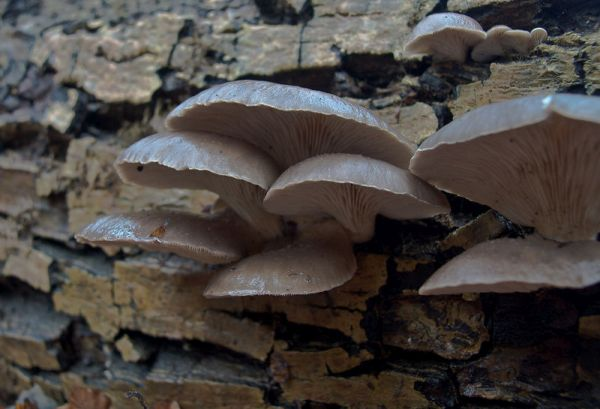
\includegraphics[width=200px]{auster3}
\caption[Austernseitling]{Austernseitling\protect\footnotemark}
\label{fig:austernseitling}
\end{figure}
\footnotetext{\cite{pilzfinder_austernseitling_image}}

\subsection{Brauner Kräuter-Seitling}
Neben dem Austernseitling ist der brauner Kräuter-Seitling ein weiterer essbarer Vertreter der Seitlinge. Er hat einen Durchmesser von 5 bis 8 cm und eine Höhe von bis zu 10 cm. Er wächst einzeln bis gruppenweise parasitisch auf absterbenden Wurzeln. In Europa ist er nur südllich der Mainlinie anzutreffen, in Deutschland sehr selten.\\
\\Der Hut des braunen Kräuter-Seitlings ist je nach Anwachsstelle kreisel- bis muschelförmig und fleischig. Der Rand ist lange eingebogen. Die Oberfläche ist kartonbraun bis rußig, matt und feinfilzig. Die Lamellen sind weiß, später creme und weit am Stiel herablaufend. Sein Geruch und Geschmack sind mild und den Austernseitling übertrifft er deutlich an Wohlgeschmack.\footcite{tintling_kraeuter}

\begin{figure}[H]
\centering
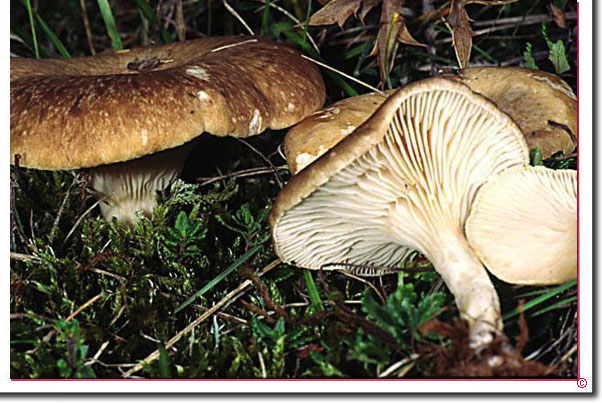
\includegraphics[width=200px]{kraeuterseitling}
\caption[Brauner Kräuter-Seitling]{Brauner Kräuter-Seitling\protect\footnotemark}
\label{fig:kraeuterseitling}
\end{figure}
\footnotetext{\cite{tintling:kraeuterseitling_image}}

\subsection{Berindeter Seitling}
Im Vergleich zum Austernseitling und Braunen Kräuter-Seitling ist der Berindete Seitling kein Speisepilz. Er wächst zwischen August und November und wird 5 bis 15 cm groß. Er ist oft in Stammwunden diverser, noch lebender Laub- und Nadelbäume zu finden. Der Pilz ist zwar verbreitet, jedoch findet man pro Fund meist nur einzelne oder wenige Fruchtkörper.\\
\\Der Hut des Berindeten Seitlings ist exzentrisch, flach ausgebreitet mit einem lange eingerolltem Rand. Die Oberfläche ist weißlich, später hellgraulich und rindenartig-derb, filzig. Später ist sie auch aufbrechend und das weiße, gilbende Hutfleisch wird freigegeben. Die Lamellen sind weiß und laufen am Stiel weit herab. Der Geruch und Geschmack ist pilzartig-würzig.\\
\\Der Pilz tritt als Wundparasit durch Verletzungen des Baumes ein. An diesen Stammwunden erscheinen dann auch die ersten Fruchkörper, oft sogar mehrere Meter über dem Erdboden. Der Pilz erzeugt dabei eine intensive Weißfäule des Kernholzes und bringt seinen Wirt auch früher oder später zum Absterben.\footcite{tintling:lungenseitling}

\begin{figure}[H]
\centering
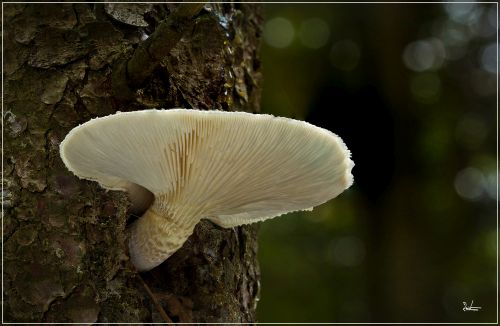
\includegraphics[width=200px]{berindeter_seitling}
\caption[Berindeter Seitling]{Berindeter Seitling\protect\footnotemark}
\label{fig:berindeter_seitling}
\end{figure}
\footnotetext{\cite{fotocom_berindeter_seitling_image}}

\subsection{Lungenseitling}
Der Lungenseitling ist ein vielerorts selten vorkommender Seitling. In Europa ist er nur lückenhaft verbreitet. Seine Hüte sind muschel- bis lungenförmig, mit anfangs eingebogenem, später scharfem Rand. Er hat einen exzentrischen Stiel und kommt in dichten, oft kiloschweren und individuenreichen Büscheln vor. Man findet ihn meistens seitlich am Holz angewachsen. Seine Oberfläche ist glatt, fettig glänzend und kittfarben bis milchkaffeebeige, sein Rand ist opak. Die Lamellen sind weiß und dünn, engstehend und untermischt. Sein Fleisch ist dick, im Stiel zäh und weiß. Der Geruch und Geschmack sind unauffällig und mild. Er ist ebenfalls essbar und mit dem Ohrförmigen Seitling verwechselbar.\footcite{tintling_berindet}

\begin{figure}[H]
\centering
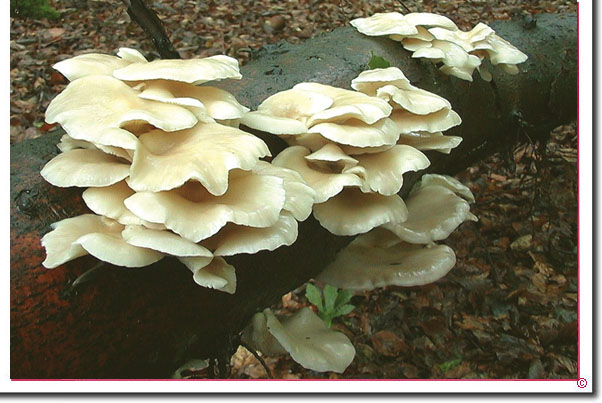
\includegraphics[width=200px]{lungenseitling}
\caption[Lungenseitling]{Lungenseitling\protect\footnotemark}
\label{fig:lungenseitling}
\end{figure}
\footnotetext{\cite{tintling:lungenseitling_image}}

%WICHTIGER ZEILENUMBRUCH IM INHALTSVERZEICHNIS
%s. http://www.latex-community.org/forum/viewtopic.php?f=5&t=4271
\addtocontents{toc}{\protect\mbox{}\protect}

\section{Medizinische Bedeutung}
Durch die in manchen Seitlingen vorhandene, antibiotisch wirkende Subtanz \emph{Pleuromulin} werden die Pilze unter anderem in der Traditionellen Chinesischen Medizin eingesetzt, zum Beispiel bei der Behandlung von Hexenschüssen und hohen Cholesterinwerten. Ebenfalls sind verschiedene Vitamine des Vitamin-B-Komplexes enthalten, die im menschlichen Organismus zur Energiegewinnung notwendig sind. Da diese Vitamine normalerweise über den Verzehr von Fleischprodukten aufgenommen werden, bieten die Seitlinge eine gute Alternative, wenn der Fleischverzehr aus ethischen oder moralischen Gründen nicht möglich ist.\\
\\Daneben gibt es noch weitere Einsatzmöglichkeiten im Bereich der Entzündungshemmung, Aufnahme von Ballaststoffen, Blutdrucksenkung und Krebsheilung.
Vor allem sind dabei die beiden Arten Austernseitling und Kräuterseitling zu nennen.\footcite{vital} Es ist jedoch anzumerken, dass nicht alle Seitlinge für die medizinische Verwendung geeignet sind.

\section{Verwechslungsmöglichkeiten}
Die Verwechslungsgefahr der Seitlinge ist vor allem zu anderen Seitlingen relativ hoch. Dadurch, dass einige Seitlingsarten essbar, andere jedoch giftig sind, ist hier äußerste Vorsicht geboten. Gerade der Ohrförmige Seitling kann zum Beispiel mit dem Speisepilz Lungenseitling (lat. \emph{Pleurotus pulmonaris}) verwechselt werden. Wer diesen nicht zu 100\% identifizieren kann, sollte ihn besser meiden und nicht verzehren, da dies unter Umständen tödliche Folgen mit sich bringen kann.\footcite{pg_ohrfoermig}\footcite{deutschlandradio}\\

\section[Rezept -- Kräuterseitlinge mit Nudeln]{Rezept -- Kräuterseitlinge mit Nudeln\footcite{rezept}}

\begin{minipage}{0.45\textwidth}

\subsection[Zutaten]{"`Zutaten}
\begin{itemize}
\item 1 Zwiebel, in Streifen
\item 1 Knoblauchzehe gepresst
\item Erdnussöl
\item 500 gr Kräuterseitlinge
\item 1 Packung Philadelphia-Kräuter, fettreduziert
\item 2 dl Rahm
\item 1 dl Cognac
\item 1 Bund Petersilie
\item 2 Salbeiblätter
\item Salz, Pfeffer
\end{itemize}
\end{minipage}%
\begin{minipage}{0.45\textwidth}
\begin{tabular}{p{\textwidth}}

\begin{figure}[H]
\centering
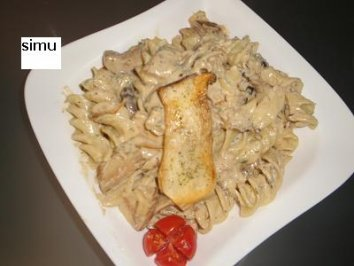
\includegraphics[width=150px]{rezept}
\caption[zubereitete Kräuterseitlinge mit Nudeln]{zubereitete Kräuterseitlinge mit Nudeln\protect\footnotemark}
\label{fig:rezept}
\end{figure}

\end{tabular}
\end{minipage}%
\footnotetext{\cite{rezept_image}}

\subsection{Zubereitung}
\begin{enumerate}
\item Die Kräuterseitlinge putzen und in mundgerechte Stücke schneiden, im Öl kräftig anbraten, Zwiebel und Knoblauch dazu geben, kurz mitbraten und mit dem Cognac ablöschen.
\item Philadelphia Rahm und kleingeschnittener Salbei dazu geben, abschmecken und weich garen.
\item Die Nudeln nach Anleitung kochen, abgiessen und zu den Pilzen geben, mischen, zuletzt die kleingehackte Petersilie dazu geben und servieren"'
\end{enumerate}

\printbibliography[heading=lit]

\end{document}
